\documentclass[tikz,border=2bp]{standalone}
\usepackage{ctex}
\usetikzlibrary{arrows.meta}
\begin{document}
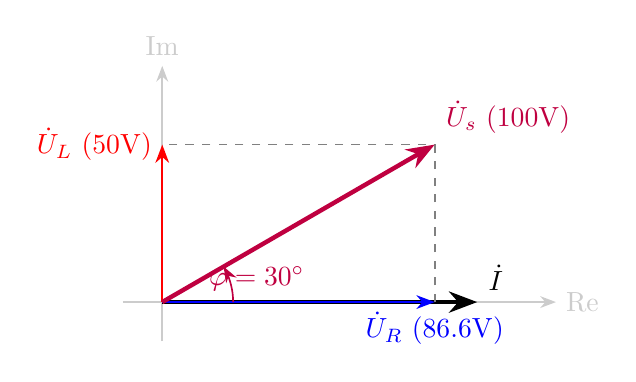
\begin{tikzpicture}[>=Stealth, semithick]
    \draw[->, gray!40] (-0.5,0) -- (5,0) node[right] {Re};
    \draw[->, gray!40] (0,-0.5) -- (0,3) node[above] {Im};
    \draw[->, ultra thick, black] (0,0) -- (4,0) node[above right] {$\dot{I}$};
    \draw[->, thick, blue] (0,0) -- (3.46,0) node[below] {$\dot{U}_R$ ($86.6\mathrm{V}$)};
    \draw[->, thick, red] (0,0) -- (0,2.0) node[left] {$\dot{U}_L$ ($50\mathrm{V}$)};
    \draw[dashed, gray] (3.46,0) -- (3.46,2.0) -- (0,2.0);
    \draw[->, ultra thick, purple] (0,0) -- (3.46,2.0) node[above right] {$\dot{U}_s$ ($100\mathrm{V}$)};
    \draw[domain=0:30, ->, purple] plot ({0.9*cos(\x)}, {0.9*sin(\x)});
    \node[purple] at (1.2,0.3) {$\varphi = 30^\circ$};
\end{tikzpicture}
\end{document}
